\documentclass[a4paper,10pt]{article}
%\usepackage[latin1]{inputenc} % Paquetes de idioma (otro encoding)
\usepackage[utf8]{inputenc} % Paquetes de idioma
\usepackage[spanish]{babel} % Paquetes de idioma
\usepackage{graphicx} % Paquete para ingresar gráficos
\usepackage{grffile}
\usepackage{hyperref}
\usepackage{fancybox}
\usepackage{amsmath}
\usepackage{amsfonts}
\usepackage{listings}
\usepackage{pdfpages}
% Paquetes de macros de Circuitos
%\usepackage{pstricks}
\usepackage{tikz}
\usepackage{color}

% Encabezado y Pié de página
% Paquete para encabezados y pie de página
\usepackage{fancyhdr} 
% Sin esta línea no se imprimiría el encabezado en todas las páginas
\pagestyle{fancy} 

% Borra el encabezado anterior (Por defecto escribe el título de la 
%  sección en la que se encuentra la hoja
\fancyhf{} 
\setlength{\headheight}{22.55pt}
\fancyhead[L]{
	{\textsf{Facultad de Ingeniería $-$ Universidad de Buenos Aires 
    \\ 75.61 Taller de Programación III}}
}
%\addtocounter{page}{5}
\fancyhead[R]{\thepage}

% Ajusta el tamaño de las líneas separadoras en el pié de página
\renewcommand{\footrulewidth}{0.4pt}
 % Ajusta el tamaño de las líneas separadoras en el encabezado
\renewcommand{\headrulewidth}{0.4pt} 

\fancyfoot[L]{
	{TP N$^{\circ}$3 - Event Managment (Google App Engine)}\\
	{\textsf{Integrantes: Torres Feyuk}}
}
		

% Carátula del Trabajo
\title{ \author{} % Lo pongo para que el warning no moleste :p
\setlength{\unitlength}{1cm} %  Especifica la unidad de trabajo
\thispagestyle{empty}

\begin{picture}(18,0)
\put(0,0){
\includegraphics[width=1.5cm, height=3cm]{Imagenes/Logo1.png}}

\put(10.5,0){
\includegraphics[width=3cm, height=3cm]{Imagenes/Logo2.png}}

\end{picture}
\\[1.5cm]
\begin{center}
	\textbf{{\Huge Facultad de Ingeniería \\ Universidad de Buenos Aires}}
    \\[2cm]
	{75.61 Taller de Programación III}\\[0.5cm]
	{TP N$^{\circ}$3 - Event Managment (Google App Engine)}\\[1.5cm]
\end{center}

\begin{flushleft}
	\textbf{Profesor: Andrés Veiga} \\
    \textbf{JTP: Pablo Roca} \\[1cm]
	\textbf{Integrantes:} \\[1cm]

	\begin{tabular}{|c|c|c|}
		\hline
		\textbf{\normalsize Padrón} & \textbf{\normalsize Nombre} 
                                    & \textbf{\normalsize Email} \\
		\hline
		\normalsize 89579 & \normalsize Torres Feyuk, Nicolás R. Ezequiel 
                          & \normalsize ezequiel.torresfeyuk@gmail.com \\
		\hline
	\end{tabular}
\end{flushleft}
\date{} % Hace que no se imprima la fecha en la cual se compilo el .tex
 }

\begin{document}
	\maketitle % Hace que el título anterior sea el principal del documento
	\newpage

    % Esta línea genera un indice a partir de las secciones y 
    % subsecciones creadas en el documento
	\tableofcontents 
	\newpage

	\section{Introducción}
		El presente trabajo práctico consiste en diseñar e implementar un sistema de recepción de eventos a través
        de la plataforma de cloud computing de google \href{http://cloud.google.com/appengine}{App Engine}. El
        presente sistema debe permitir el ingreso de personas invitadas en diferentes eventos, como asi también
        tener la posibilidad de poder consultar quienes son los invitados anotados en cada uno de ellos.
          
         
    \section{Desarrollo}
        Google App Engine permite realizar el desarrollo de las aplicaciones web a través de los siguientes 
        lenguajes de programación:

        \begin{itemize}
            \item Java
            \item Python
            \item Go
            \item PHP
        \end{itemize}

        Debido a la simplicidad del lenguaje y la falta de conocimientos en las otras opciones, se decidió implementar
        el sistema en Python. App Engine permite realizar el desarrollo de la parte Servidor a través de cualquier
        web framework de Python que implemente la interfaz WSGI(Web Service Gateway Interface). Se lista a continuación
        algunos de los frameworks que cumplen con esta especificación:
        
        \begin{itemize}
            \item Django
            \item CherryPy
            \item Pylon 
            \item web.py
            \item web2pyi
            \item webapp2
        \end{itemize}

        Para realizar la presente aplicación se decidió utilizar \text{webapp2}. El motivo de esta elección es que
        la complejidad del presente proyecto era baja y los tutoriales de google respecto a las aplicaciones de 
        Python para App Engine están desarrolladas con este framework. \\
        \indent Para el desarrollo y diseño de la página web se utilizó HTML, scripts en Javascript y JQuery 
        y el template language Jinja2. Este último fue utilizado la generación dinámica de la página principal del 
        proyecto, la cual nuevamente se realizó en función del 
        \href{https://cloud.google.com/appengine/docs/python/gettingstartedpython27/introduction}{tutorial de App Engine}.
        

    \newpage
    \section{Arquitectura 4 + 1}
    \subsection{Casos de Uso}
        En la figura \ref{DiagCU} se exhibe el diagrama de casos de uso del sistema. Se detalla a continuación cada
        una de las entradas del mismo:

        \begin{figure}[!Hhtb]                                             
            \centering                                                   
            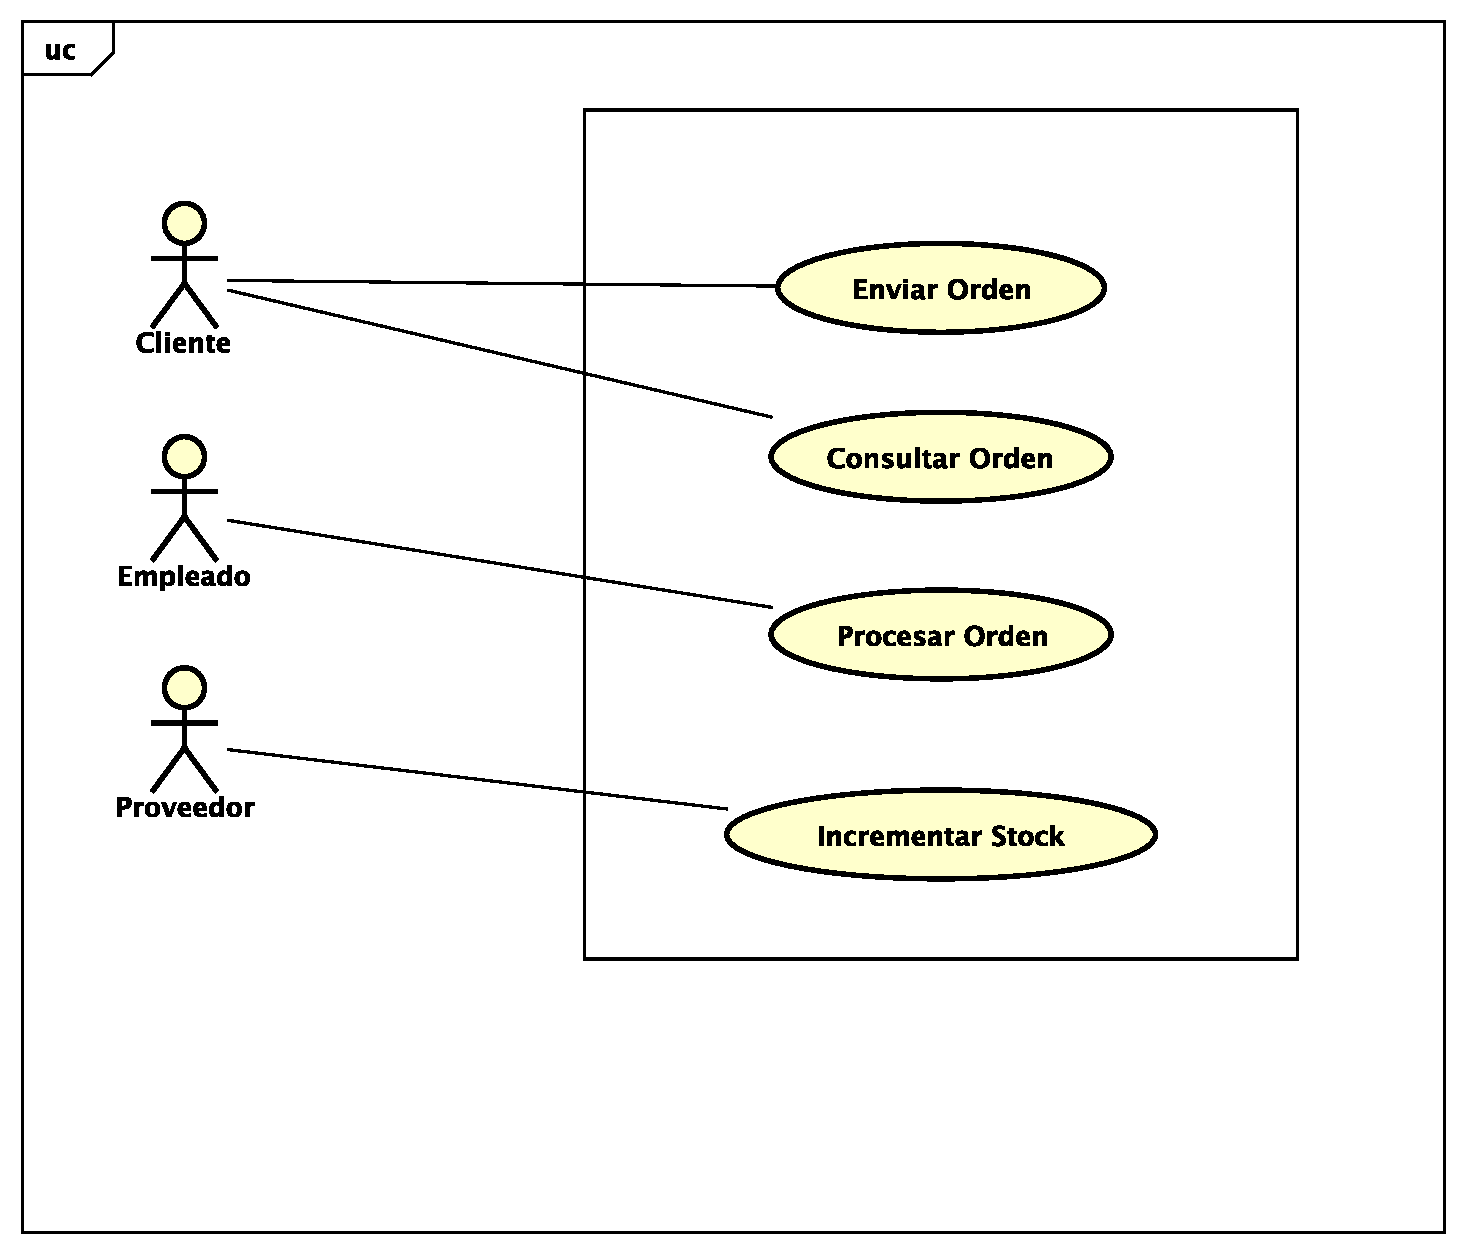
\includegraphics[width=15cm,origin=c]{Imagenes/Casos_De_Uso.pdf}        
            \caption{Diagrama de Casos de Uso} \label{DiagCU}
        \end{figure}

        \begin{itemize}
            \item \textbf{Suscribir Invitado:} Un invitado ingresa sus datos pertinentes a la página web e intenta
            registrarse. El sistema toma como identificador único del usuario su email, por lo cual en el caso de
            que ya exista una persona en el mismo evento con el mismo email, la invitación será rechazada.
            \item \textbf{Consultar Invitados:} Un usuario administrador o invitado elige el evento a consultar. Al 
            hacerlo, la página web muestra en una tabla la lista de invitados actual del evento.  
            \item \textbf{Crear Evento:} Un usuario administrador crea un evento e ingresa el nombre y la 
            máxima cantidad de invitados del mismo.  
            \item \textbf{Borrar Evento:} Un usuario administrador posicionado sobre un evento específico elimina 
            al mismo. Al hacer esto, se borrará del storage de la aplicación el evento junto con todos los invitados
            registrados en el mismo.
            \end{itemize}

        Cabe destacar que no existe el caso de uso \textbf{Desuscribir Invitado} debido a que el enunciado no 
        especificaba este caso. El caso \textbf{Borrar Evento} fue agregado solamente para poder eliminar fácilmente
        aquellos eventos creados a partir de pruebas de carga.


    \newpage
    \subsection{Vista Lógica}
        En la figura \ref{DiagClases} se exhibe el diagrama de clases, el cual muestra la vista lógica del sistema. 
        A continuación se adjunta una breve explicación de cada una de las clases:

        \begin{figure}[!Hhtb]                                             
            \centering                                                   
            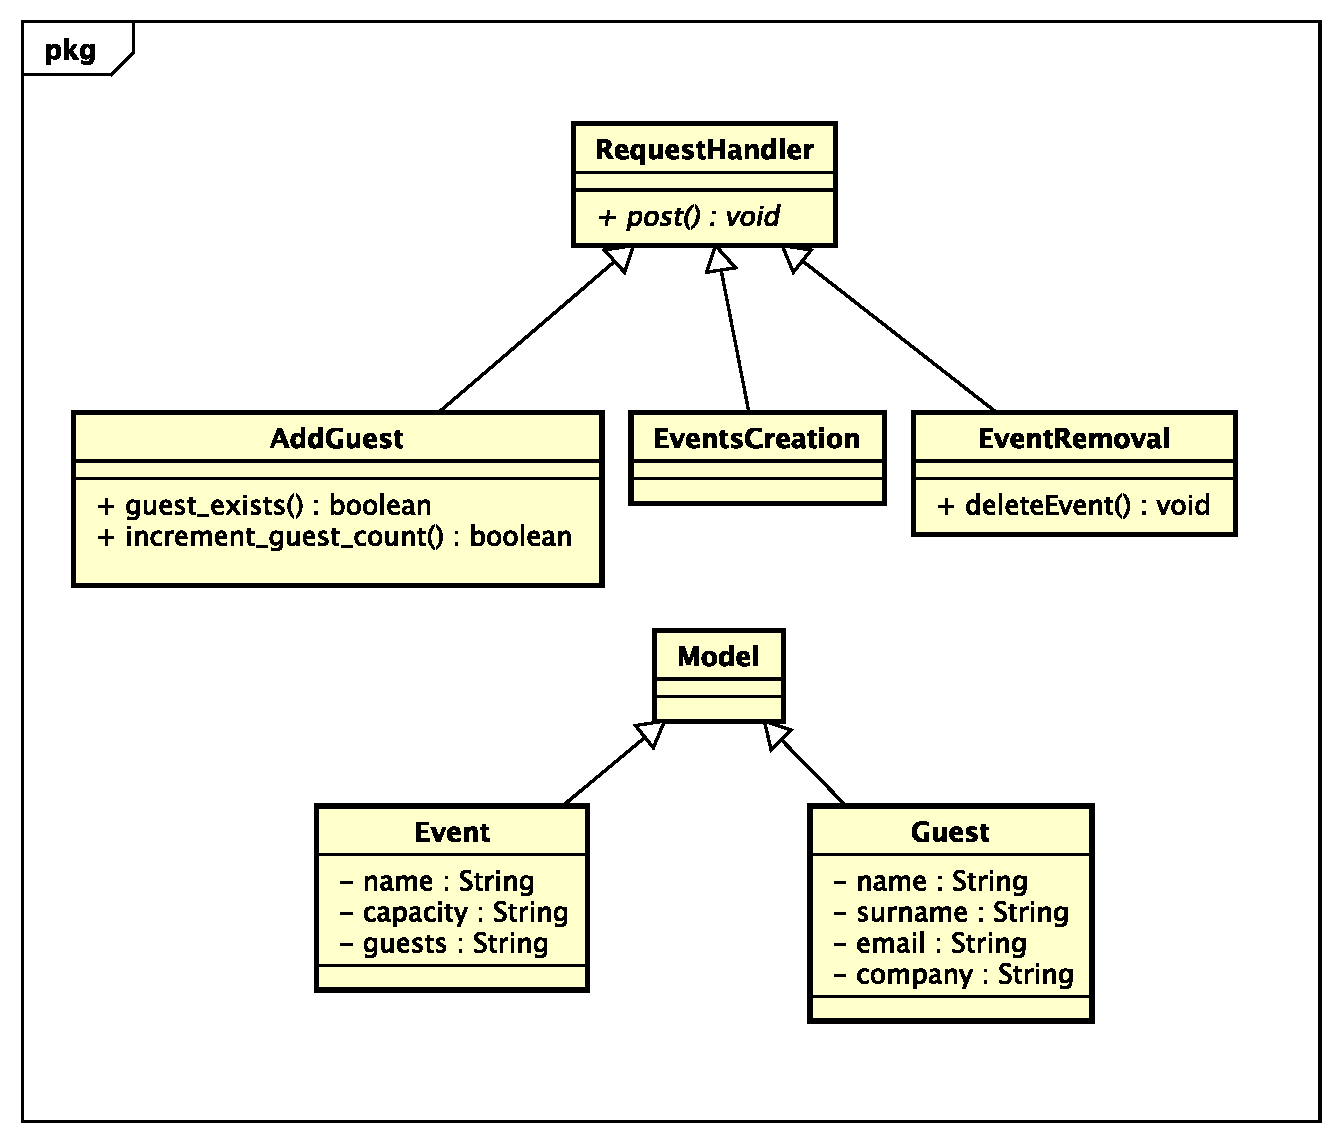
\includegraphics[width=15cm,origin=c]{Imagenes/Clases.pdf}        
            \caption{Diagrama de Clases} \label{DiagClases}
        \end{figure}

        \begin{itemize}
            \item \textbf{AddGuest:} Clase derivada de RequestHandler. Al recibir un post, se encarga de validar
            que el invitado a ingresar no exista y luego agrega al mismo. Además, chequea si el evento permite
            ingresar más invitados anter de dar el alta.
            \item \textbf{EventsCreation:} Clase que deriva de RequestHandler. Al recibir un post, crea un evento
            nuevo en el datastorage
            \item \textbf{EventRemoval:} Clase que deriva de RequestHandler. Al recibir un post, obtiene el evento
            pasado por parámetro y elimina al mismo junto con todos los invitados asociados.
            \item \textbf{Event:} Objeto que represeta a un evento en el datastorage.
            \item \textbf{Guest:} Objeto que representa a un invitado en el datastorage.
        \end{itemize}

    % \newpage
    % \subsection{Vista de Procesos}

    % \newpage
    % \subsection{Vista Física}

    \newpage
    \section{Pruebas de Carga}
        La aplicación en la nube se puede acceder a través del siguiente \href{https://poised-throne-110314.appspot.com}{link} 
        a través de HTTPS: poised-throne-110314.appspot.com.
        Para probar la performance de la misma, se investigaron diferentes simuladores de carga. Los requisitos del  
        simulador a buscar son los siguientes:

        \begin{itemize}
            \item \textbf{Simplicidad:} La aplicación a testear es muy sencilla. Solo se desea enviar un POST al 
            servidor con ciertos datos y analizar como responde el mismo. 
            \item \textbf{Flexibilidad:}El simulador debe tener la capacidad de poder recibir un conjunto de tests y 
            ejecutar los mismos de forma automática.
            \item \textbf{Concurrencia:} El simulador debe poder lanzar los tests desde N procesos/threads diferentes, 
            para poder probar la concurrencia del sistema Web.
        \end{itemize}

        Se detallan a continuación las características de los simuladores investigados:

        \subsection{Jmeter}
            \href{http://http://jmeter.apache.org}{Apache Jmeter} es un simulador desarrollado por la Apache Software
            Foundation. Es un completo simulador que permite realizar pruebas de carga complejas utilizando diferentes

        \subsection{The Grinder}
            \begin{itemize}
            \end{itemize}

        \subsection{The Grinder}
            \begin{itemize}
            \end{itemize}

        Los primeros simuladores a probar fueron \href{http://http://jmeter.apache.org}{Jmeter} y 
        \href{http://grinder.sourceforge.net}{The Grinder}. Jmeter fue descartado inmediatamente al abrir la 
        documentación la cual posee más de 500 hojas. Claramente este simulador no cumple el requisito de 
        \textit{Simplicidad} que se estaba buscando. Luego se realizaron pruebas con \textit{The Grinder}. Este 
        simulador resultó ser más ameno debido a que los tests se programan en Jython. Se intentó utilizar el
        mismo pero luego de estar una hora sin obtener resultados concretos, se decidió buscar otra alternativa. \\
        \indent Buscando se encontró \href{http://www.pylot.org/}{Pylot}. El mismo es un simulador de carga que 
        recibe los tests a través de un xml y con el cual se modificar parámetros de carga a través de un 
        archivo de configuración. Se muestra a continuación un XML de ejemplo de la simulación de un HTTPRequest. 

        \vspace{1cm}
        \lstset{language=XML}
        \begin{lstlisting}
<testcases>
  <case>
    <url>http://localhost:8080/add_guest</url>
    <method>POST</method>
    <body><![CDATA[actualEvent=Mondongo]]></body>
  </case>
</testcases>
        \end{lstlisting}

        \vspace{1cm}
        \noindent El simulador posee los siguientes parámetros a configurar:
        \begin{itemize}
            \item \textbf{Agents:} Cantidad de threads a lanzar para realizar las simulaciones.
            \item \textbf{Duration:} Duración (en segundos) de la simulación.
            \item \textbf{RampUp:} Tiempo (en segundos) a esperar entre el lanzamiento de un agente y el proximo.
            \item \textbf{Interval:} Periodicidad con la cual un agente realiza un test en función de las pruebas
            almacenadas en el XML.
        \end{itemize}

        \subsection{Resultados}
            Se muestra a continuación los resultados de las pruebas de cargas realizadas. En las mismas se muestra
            como se fueron modificando los parámetros del simulador, junto con la respuesta de la WebApp. 

            \vspace{1cm}
            \hspace*{-3cm} 
            \begin{tabular}{|c|c|c|c|c|c|c|}
                \hline
                \textbf{Agentes} & \textbf{Duración (seg)} & \textbf{RampUp(ms)} & \textbf{Interval(ms)} & \textbf{Resp. Time (ms)} & \textbf{Requests} & \textbf{Errors} \\
                \hline
                1 & 30 & 0 & 500 & 452 & 57 & 0 \\
                \hline 
                1 & 30 & 0 & 100 & 478 & 61 & 0 \\
                \hline 
                5 & 30 & 0 & 100 & 567 & 237 & 0 \\
                \hline 
                10 & 30 & 0 & 100 & 1194 & 226 & 37 \\
                \hline 
                15 & 30 & 0 & 100 & 1390 & 256 & 78 \\
                \hline 
            \end{tabular}

\end{document}
        
